\subsection{Exemples de comparaisons de transcriptions pour la batterie}
\textit{drummer\_01/session3 — 10\_rock-folk\_90\_beat\_4-4}\\\\
Fichier midi vers partition avec musescore $\Rightarrow$ Transcription manuelle\\
\includegraphics[height=20mm, width=50mm]{z_images/transcriptions_manuelles/0_prise_en_main/0_tests_drummer_01__session3/musescore_0.png}\ \ \ \ 
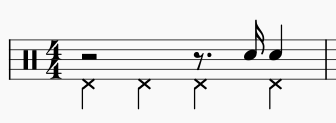
\includegraphics[height=20mm, width=55mm]{z_images/transcriptions_manuelles/0_prise_en_main/0_tests_drummer_01__session3/manuel_0.png}
\begin{itemize}
	\item Erreur d’indication de mesure ;
	\item Mauvaise transcription d’une noire.\\
\end{itemize}
La noire du 4ème temps se retrouve sur le premier temps de la mesure suivante et elle se transforme en un triolet de double croches dont seules les deux premières seraient jouées.\\\\
\textit{drummer\_01/session3 — 10\_rock-folk\_90\_beat\_4-4}\\\\
Fichier midi vers partition avec musescore $\Rightarrow$ Transcription manuelle\\
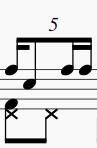
\includegraphics[height=20mm, width=15mm]{z_images/transcriptions_manuelles/0_prise_en_main/0_tests_drummer_01__session3/musescore_1.png}\ \ \ \ 
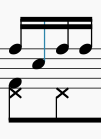
\includegraphics[height=20mm, width=15mm]{z_images/transcriptions_manuelles/0_prise_en_main/0_tests_drummer_01__session3/manuel_1.png}\\
\begin{itemize}
	\item Erreur de quantification : les doubles croches ont été interprétées en quintolet;\\
\end{itemize}
drummer\_01/session3 — 2\_jazz-swing\_185\_beat\_4-4
\\\\
Fichier midi vers partition avec musescore $\Rightarrow$ Transcription manuelle\\
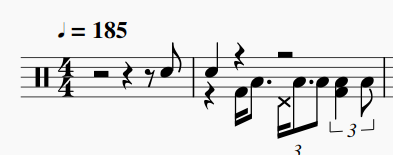
\includegraphics[height=25mm, width=60mm]{z_images/transcriptions_manuelles/0_prise_en_main/0_tests_drummer_01__session3/musescore_2.png}\ \ \ \ 
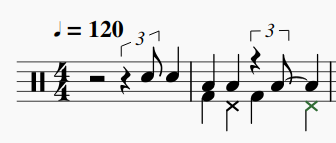
\includegraphics[height=25mm, width=55mm]{z_images/transcriptions_manuelles/0_prise_en_main/0_tests_drummer_01__session3/manuel_2.png}
\begin{itemize}
	\item L’indication de mesure est correcte mais tout a été décalé d’un temps car la première noire sur la caisse claire est jouée sur le 4ème temps et non sur le premier temps de la deuxième mesure comme l’indique la transcription de musescore.
	\item Les toms basses des 1er et 2ème temps de la mesure musescore auraient dû être sur les temps et non décalés d’une double croche vers la droite.\\
\end{itemize}
drummer\_01/session1 — 1\_funk\_80\_beat\_4-4\\\\
Fichier midi vers partition avec musescore $\Rightarrow$ Transcription manuelle\\
\includegraphics[height=25mm, width=40mm]{z_images/transcriptions_manuelles/0_prise_en_main/1_drummer_01__session1/musescore_0.png}\ \ \ \ 
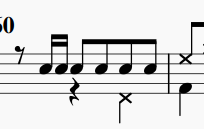
\includegraphics[height=25mm, width=40mm]{z_images/transcriptions_manuelles/0_prise_en_main/1_drummer_01__session1/Manuelle_0.png}
\begin{itemize}
	\item On dirait que lorsque certaines notes sont proches, elles se resserrent et suppriment celles qui aurait dû être sur le temps.\\
\end{itemize}
%drummer\_01/session1 — 1\_funk\_80\_beat\_4-4\\
%Fichier midi vers partition avec musescore :\\\\
%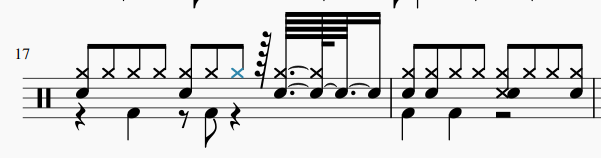
\includegraphics[height=25mm, width=80mm]{z_images/transcriptions_manuelles/0_prise_en_main/1_drummer_01__session1/MuseScore_1.png} \\\\
%Transcription manuelle :\\
%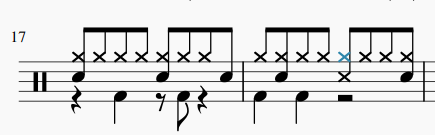
\includegraphics[height=20mm, width=65mm]{z_images/transcriptions_manuelles/0_prise_en_main/1_drummer_01__session1/Manuelle_1.png} \\
%\begin{itemize}
%	\item La caisse claire de la 2ème croche du 4ème temps de la 1ère mesure se transforme en une combinaison de quadruple/quintuple/double croches liées qui commence par un soupir et finit en débordant sur le premier temps de la mesure suivante. 
%\end{itemize}
\subsubsection{Exemple avec des flas}
%Des exemples de notation flas tom/caisse-claire existent dans des partitions récentes (rythmique binaire J.-F. Juskowiak).\\
%$\Rightarrow$ Ils faudra donc les prendre en compte dans les comparaisons de transcriptions.
Fichier midi vers partition avec musescore :\\
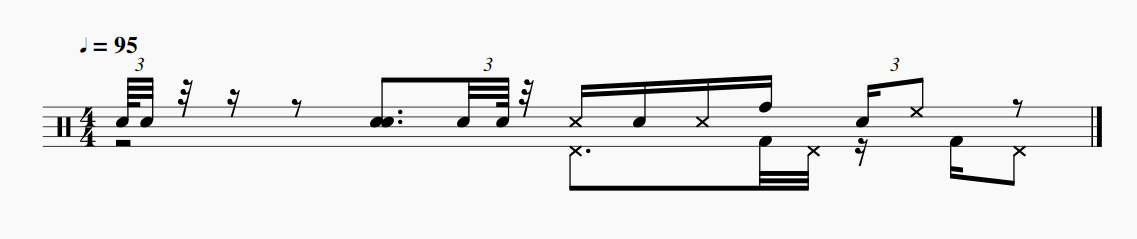
\includegraphics[height=30mm, width=120mm]{z_images/transcriptions_manuelles/1_transcriptions_flas/124_funk_95_fill_4-4_0.png}\\
Transcription manuelle :\\
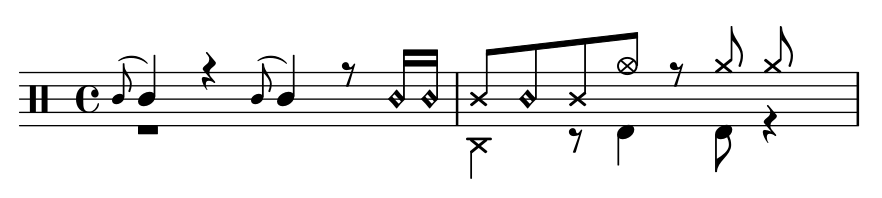
\includegraphics[height=20mm, width=90mm]{z_images/transcriptions_manuelles/1_transcriptions_flas/124_funk_95_fill_4-4_1_.png}\\